\chapter{Mécanismes réactionnels~: actes élémentaires et approximations}\label{ch:b1:elementary-steps}

Le monoxyde d'azote, formé dans les moteurs automobiles et par la
foudre, se combine au dioxygène de l'air~: \ce{2NO + O2 -> 2NO2}. Mesurée
au laboratoire, la vitesse de cette réaction est proportionnelle à
$[\ce{NO}]^2[\ce{O2}]$ --- et elle est \emph{plus lente} quand on chauffe
le gaz. Un choc unique entre trois molécules pourrait expliquer le
premier fait, jamais le second~: tout choc devient plus énergétique avec
la température. L'explication est que la réaction n'est pas un événement
unique mais une suite d'événements plus simples, son mécanisme. Ce
chapitre définit ces \omterm{def:b1:elementary-steps:elementary-step}{actes élémentaires}, le \omterm{def:b1:elementary-steps:energy-profile}{profil énergétique} le long
duquel ils se déroulent et les approximations qui transforment un
mécanisme en \omterm{def:b1:rate-laws:order}{loi de vitesse}~; il se termine par la catalyse, l'art
d'ouvrir un chemin plus facile.

\begin{recall}
Le livre 1 (année 12) a décrit un \omterm{def:b1:elementary-steps:elementary-step}{mécanisme réactionnel} comme une suite
d'étapes dessinées avec des flèches courbes, au cours desquelles des
intermédiaires se forment et se consomment, et un \omterm{def:b1:elementary-steps:catalyst}{catalyseur} comme une
espèce qui accélère une réaction sans être consommée. Les \omterm{def:b1:rate-laws:order}{lois de
vitesse}, les ordres et la \omterm{thm:b1:rate-laws:arrhenius}{loi d'Arrhenius} ont été définis au
\cref{ch:b1:rate-laws}.
\end{recall}

\section{Actes élémentaires}

\begin{definition}[Acte élémentaire, molécularité, mécanisme]\label{def:b1:elementary-steps:elementary-step}
Un \emph{acte élémentaire}\index{acte elementaire@acte élémentaire} est une réaction qui se produit en un seul
événement moléculaire, tel qu'il est écrit, sans aucun intermédiaire. Sa
\emph{molécularité}\index{molecularite@molécularité} est le nombre de particules qui réagissent dans
cet événement~: 1 (monomoléculaire, une décomposition ou un
réarrangement), 2 (bimoléculaire, un choc), rarement 3. Un
\emph{mécanisme réactionnel}\index{mecanisme reactionnel@mécanisme réactionnel} est l'ensemble des actes élémentaires
dont la somme est la réaction globale. Une espèce formée dans un acte et
consommée dans un acte ultérieur, absente de l'équation globale, est un
\emph{intermédiaire réactionnel}\index{intermediaire reactionnel@intermédiaire réactionnel}.
\end{definition}

\begin{proposition}[Loi de vitesse d'un acte élémentaire]\label{prop:b1:elementary-steps:elementary-law}
Un \omterm{def:b1:elementary-steps:elementary-step}{acte élémentaire} admet un ordre, et ses \omterm{def:b1:rate-laws:order}{ordres partiels} sont égaux à
ses coefficients stœchiométriques~: $\mathrm{A} \to \dots$ a pour
vitesse $v = k[\mathrm{A}]$~;
$\mathrm{A} + \mathrm{B} \to \dots$ a pour vitesse $v = k[\mathrm{A}][\mathrm{B}]$~;
$2\,\mathrm{A} \to \dots$ a pour vitesse $v = k[\mathrm{A}]^2$. La
réciproque est fausse~: une réaction dont les ordres sont égaux aux
coefficients n'est pas nécessairement élémentaire.
\end{proposition}

\begin{proof}[Raisonnement]
Un acte bimoléculaire se produit quand un \ce{A} rencontre un \ce{B}~;
le nombre de telles rencontres par unité de volume et de temps est
proportionnel au nombre de \ce{A} par unité de volume et au nombre de
\ce{B}, donc à
$[\ce{A}][\ce{B}]$. Un acte monomoléculaire arrive à chaque molécule avec
une probabilité fixe par unité de temps, d'où une vitesse
proportionnelle à $[\ce{A}]$.
\end{proof}

\begin{remark}[Pourquoi la molécularité dépasse rarement deux]\label{rem:b1:elementary-steps:termolecular}
La rencontre simultanée de trois particules, chacune avec l'énergie et
l'orientation convenables, est un événement rare~; une réaction d'\omterm{def:b1:rate-laws:order}{ordre
global} 3 résulte presque toujours de deux actes bimoléculaires
successifs, comme dans le problème du week-end.
\end{remark}

\section{Profils énergétiques}

\begin{definition}[Coordonnée réactionnelle, profil énergétique, état de transition]\label{def:b1:elementary-steps:energy-profile}
Au cours d'un \omterm{def:b1:elementary-steps:elementary-step}{acte élémentaire}, les atomes passent de la disposition des
réactifs à celle des produits~; une variable qui mesure cette
progression (une longueur de liaison qui augmente, une autre qui
diminue) est la \emph{coordonnée
réactionnelle}\index{coordonnee reactionnelle@coordonnée réactionnelle}. La courbe de l'énergie potentielle du
système le long de cette coordonnée est le \emph{profil
énergétique}\index{profil energetique@profil énergétique}. Son maximum est l'\emph{état de transition}\index{etat de transition@état de transition},
une disposition des atomes où des liaisons sont à moitié formées et à
moitié rompues, qui ne dure pas plus longtemps qu'une vibration
moléculaire et ne peut pas être isolée. La hauteur de ce maximum
au-dessus des réactifs est la barrière énergétique de l'acte.
\end{definition}

\begin{omfigure}
\begin{tikzpicture}
\begin{axis}[omprofile, name=a,
  width=0.48\linewidth, height=5.4cm, xmin=0, xmax=10, ymin=-68, ymax=95,
  xlabel={coordonnée réactionnelle}, ylabel={énergie}]
\addplot[omDef, very thick] table[x=x, y=E] {figdata/out/bachelor-1-energy-profiles-one-step.dat};
\draw[dashed, black!40] (axis cs:0,0) -- (axis cs:10,0);
\draw[<->, omThm] (axis cs:5,0) -- (axis cs:5,79);
\node[omThm, anchor=west, font=\small] at (axis cs:5.1,30) {barrière};
\draw[<->, omProp] (axis cs:9.9,0) -- (axis cs:9.9,-40);
\node[omProp, anchor=east, font=\small] at (axis cs:9.8,-14) {$\Delta E$};
\node[anchor=south, font=\small] at (axis cs:5,81) {état de transition};
\node[anchor=north west, font=\small] at (axis cs:0.15,-3) {réactifs};
\node[anchor=north, font=\small] at (axis cs:8.6,-42) {produits};
\end{axis}
\begin{axis}[omprofile, at={(a.east)}, anchor=west, xshift=1.2cm,
  width=0.48\linewidth, height=5.4cm, xmin=0, xmax=10, ymin=-64, ymax=95,
  xlabel={coordonnée réactionnelle}, ylabel={énergie}]
\addplot[omDef, very thick] table[x=x, y=E] {figdata/out/bachelor-1-energy-profiles-two-step.dat};
\node[anchor=south, font=\small] at (axis cs:3,71) {ET 1};
\node[anchor=south, font=\small] at (axis cs:7,56) {ET 2};
\node[anchor=north, font=\small, align=center] at (axis cs:5,27) {inter-\\médiaire};
\node[anchor=north west, font=\small] at (axis cs:0.15,-3) {réactifs};
\node[anchor=north east, font=\small] at (axis cs:10,-43) {produits};
\end{axis}
\end{tikzpicture}

{\small À gauche~: le profil d'un \omterm{def:b1:elementary-steps:elementary-step}{acte élémentaire}, avec sa barrière et
la variation d'énergie de la réaction. À droite~: un mécanisme en deux
actes~; l'intermédiaire se trouve dans un creux entre deux \omterm{def:b1:elementary-steps:energy-profile}{états de
transition} (ET). Les énergies sont indicatives.}
\end{omfigure}

\begin{proposition}[Barrières et loi d'Arrhenius]\label{prop:b1:elementary-steps:barrier}
L'\omterm{def:b1:rate-laws:activation-energy}{énergie d'activation} d'un \omterm{def:b1:elementary-steps:elementary-step}{acte élémentaire} est voisine de sa
barrière~: seuls les chocs qui apportent au moins cette énergie
atteignent l'\omterm{def:b1:elementary-steps:energy-profile}{état de transition}. Pour les sens direct et inverse d'un
acte, $E_{a,+} -
E_{a,-} = \Delta E$, l'énergie de réaction de l'acte.
\end{proposition}

\begin{proof}[Raisonnement]
L'acte inverse franchit la même barrière par l'autre versant~: sa
hauteur mesurée à partir des produits dépasse celle du sens direct de
$-\Delta E$.
\end{proof}

\begin{proposition}[Le postulat de Hammond]\label{prop:b1:elementary-steps:hammond}
L'\omterm{def:b1:elementary-steps:energy-profile}{état de transition} d'un \omterm{def:b1:elementary-steps:elementary-step}{acte élémentaire} ressemble, par sa structure
et son énergie, à l'espèce dont il est le plus proche en énergie~: aux
produits pour un acte fortement endothermique, aux réactifs pour un acte
fortement exothermique. Par conséquent, pour un acte qui forme un
intermédiaire de haute énergie, tout ce qui stabilise l'intermédiaire
abaisse aussi la barrière qui y mène.
\end{proposition}
\admitted

\section{Étape cinétiquement déterminante et pré-équilibre}

\begin{definition}[Étape cinétiquement déterminante]\label{def:b1:elementary-steps:rds}
Dans une suite d'actes, l'\emph{étape cinétiquement
déterminante}\index{etape cinetiquement determinante@étape cinétiquement déterminante} est un acte beaucoup plus lent que tous les
autres~; la vitesse globale est égale à sa vitesse, les actes plus
rapides s'y ajustant comme les voitures d'une route suivent le rythme
de son point le plus lent.
\end{definition}

\begin{definition}[Approximation du pré-équilibre rapide]\label{def:b1:elementary-steps:pre-equilibrium}
Dans l'\emph{approximation du pré-équilibre rapide}\index{approximation du pre-equilibre rapide@approximation du pré-équilibre rapide},
on suppose qu'un acte rapide et renversable qui précède l'\omterm{def:b1:elementary-steps:rds}{étape
cinétiquement déterminante} reste à l'équilibre tout du long~: les
concentrations de ses espèces vérifient sa constante d'équilibre
$K_1 = k_1/k_{-1}$.
\end{definition}

\begin{proposition}[Loi de vitesse issue d'un pré-équilibre]\label{prop:b1:elementary-steps:pre-equilibrium-law}
Pour le mécanisme
\[
  \mathrm{A} + \mathrm{B} \underset{k_{-1}}{\overset{k_1}{\rightleftharpoons}} \mathrm{I}
  \ \text{(rapide)}, \qquad
  \mathrm{I} + \mathrm{C} \xrightarrow{\ k_2\ } \mathrm{P} \ \text{(lent)},
\]
la vitesse vaut $v = k_2K_1[\mathrm{A}][\mathrm{B}][\mathrm{C}]$, d'\omterm{def:b1:rate-laws:order}{ordre
global} 3, avec la constante apparente $k = k_1k_2/k_{-1}$.
\end{proposition}

\begin{proof}
La vitesse est celle de l'acte lent, $v = k_2[\mathrm{I}][\mathrm{C}]$.
Le premier acte reste à l'équilibre~: $k_1[\mathrm{A}][\mathrm{B}] =
k_{-1}[\mathrm{I}]$, donc $[\mathrm{I}] = K_1[\mathrm{A}][\mathrm{B}]$.
La substitution donne le résultat.
\end{proof}

\section{L'approximation des états quasi stationnaires}

\begin{theorem}[Réactions successives d'ordre 1]\label{thm:b1:elementary-steps:consecutive}
Pour $\mathrm{A} \xrightarrow{k_1} \mathrm{B} \xrightarrow{k_2} \mathrm{C}$,
les deux actes étant d'ordre 1, avec $[\mathrm{A}] = a_0$ et $[\mathrm{B}] =
[\mathrm{C}] = 0$ à $t = 0$ et $k_1 \ne k_2$~:
\[
  [\mathrm{A}] = a_0\eu^{-k_1t}, \qquad
  [\mathrm{B}] = \frac{a_0k_1}{k_2 - k_1}\big(\eu^{-k_1t} - \eu^{-k_2t}\big),
  \qquad [\mathrm{C}] = a_0 - [\mathrm{A}] - [\mathrm{B}] .
\]
L'intermédiaire passe par un maximum à $t_{\max} = \dfrac{\ln(k_2/k_1)}
{k_2 - k_1}$.
\end{theorem}

\begin{proof}
$\dd[\mathrm{A}]/\dd t = -k_1[\mathrm{A}]$ donne $[\mathrm{A}]$. Ensuite,
$\dd[\mathrm{B}]/\dd t + k_2[\mathrm{B}] = k_1a_0\eu^{-k_1t}$, équation
linéaire du premier ordre~: en multipliant par $\eu^{k_2t}$, $\frac{\dd}{\dd t}
\big([\mathrm{B}]\eu^{k_2t}\big) = k_1a_0\eu^{(k_2-k_1)t}$, dont
l'intégrale à partir de 0, où $[\mathrm{B}] = 0$, est $[\mathrm{B}]\eu^{k_2t} =
\frac{k_1a_0}{k_2-k_1}(\eu^{(k_2-k_1)t} - 1)$. La conservation de la
matière donne
$[\mathrm{C}]$. La dérivée de $[\mathrm{B}]$ s'annule quand $k_1\eu^{-k_1t}
= k_2\eu^{-k_2t}$, c'est-à-dire en $t_{\max}$.
\end{proof}

\begin{definition}[Approximation des états quasi stationnaires]\label{def:b1:elementary-steps:qssa}
Dans l'\emph{approximation des états quasi stationnaires}\index{approximation des etats quasi stationnaires@approximation des états quasi stationnaires}
(AEQS), la concentration d'un intermédiaire très réactif, consommé
beaucoup plus vite qu'il n'est formé, est considérée comme constante et
faible après une courte période d'induction~: sa \omterm{def:b1:rate-laws:rate}{vitesse de formation}
est égale à sa vitesse de consommation,
$\dd[\mathrm{I}]/\dd t \approx 0$.
\end{definition}

\begin{proposition}[Quand l'état quasi stationnaire est valable]\label{prop:b1:elementary-steps:qssa-justified}
Pour $\mathrm{A} \to \mathrm{B} \to \mathrm{C}$ avec $k_2 \gg k_1$~: au
bout d'une durée de l'ordre de $1/k_2$, $[\mathrm{B}] \approx k_1[\mathrm{A}]/k_2$
(ce que donne $\dd[\mathrm{B}]/\dd t = 0$), $[\mathrm{B}]$ reste faible,
et le produit se forme à la vitesse $\dd[\mathrm{C}]/\dd t \approx k_1[\mathrm{A}]$~:
le premier acte est cinétiquement déterminant.
\end{proposition}

\begin{proof}
Pour $k_2 \gg k_1$ et $t \gg 1/k_2$, $\eu^{-k_2t}$ est négligeable
devant
$\eu^{-k_1t}$ et $k_2 - k_1 \approx k_2$, donc $[\mathrm{B}] \approx (a_0k_1/k_2)
\eu^{-k_1t} = k_1[\mathrm{A}]/k_2 \ll [\mathrm{A}]$. Alors
$\dd[\mathrm{C}]/\dd t = k_2[\mathrm{B}] \approx k_1[\mathrm{A}]$.
\end{proof}

\begin{omfigure}
\begin{tikzpicture}
\begin{axis}[name=s,
  width=0.48\linewidth, height=5.2cm, xmin=0, xmax=6, ymin=0, ymax=1.05,
  axis x line=bottom, axis y line=left,
  xlabel={$k_1t$}, ylabel={concentration$/a_0$},
  title={$k_2 = 0.5\,k_1$}, title style={font=\small},
  tick label style={font=\small}, label style={font=\small}]
\addplot[omDef, thick] table[x=t, y=a] {figdata/out/bachelor-1-consecutive-reactions-slow.dat};
\addplot[omThm, thick] table[x=t, y=b] {figdata/out/bachelor-1-consecutive-reactions-slow.dat};
\addplot[omMeth, thick] table[x=t, y=c] {figdata/out/bachelor-1-consecutive-reactions-slow.dat};
\node[omDef, font=\small, anchor=west] at (axis cs:0.4,0.75) {A};
\node[omThm, font=\small, anchor=south] at (axis cs:1.39,0.51) {B};
\node[omMeth, font=\small, anchor=west] at (axis cs:4.5,0.75) {C};
\end{axis}
\begin{axis}[at={(s.east)}, anchor=west, xshift=1.2cm,
  width=0.48\linewidth, height=5.2cm, xmin=0, xmax=6, ymin=0, ymax=1.05,
  axis x line=bottom, axis y line=left,
  xlabel={$k_1t$}, ylabel={concentration$/a_0$},
  title={$k_2 = 20\,k_1$}, title style={font=\small},
  tick label style={font=\small}, label style={font=\small}]
\addplot[omDef, thick] table[x=t, y=a] {figdata/out/bachelor-1-consecutive-reactions-fast.dat};
\addplot[omThm, thick] table[x=t, y=b] {figdata/out/bachelor-1-consecutive-reactions-fast.dat};
\addplot[omMeth, thick] table[x=t, y=c] {figdata/out/bachelor-1-consecutive-reactions-fast.dat};
\addplot[black, dashed] table[x=t, y=bss] {figdata/out/bachelor-1-consecutive-reactions-fast.dat};
\node[omDef, font=\small, anchor=west] at (axis cs:1.4,0.32) {A};
\node[omThm, font=\small, anchor=south west] at (axis cs:2,0.22) {B (AEQS en tirets)};
\node[omMeth, font=\small, anchor=west] at (axis cs:4.5,0.85) {C};
\end{axis}
\end{tikzpicture}

{\small Réactions successives $\mathrm{A} \to \mathrm{B} \to \mathrm{C}$.
À gauche~: l'intermédiaire s'accumule et passe par un maximum en
$k_1t = 1.39$. À droite~: lorsqu'il est consommé vingt fois plus vite
qu'il ne se forme, il reste faible et suit la valeur quasi stationnaire
$k_1[\mathrm{A}]/k_2$ (tirets) après une brève période d'induction.}
\end{omfigure}

\begin{method}[Loi de vitesse d'un mécanisme]\label{met:b1:elementary-steps:rate-law}
Pour établir la \omterm{def:b1:rate-laws:order}{loi de vitesse} d'un mécanisme~:
\begin{enumerate}
  \item écrire la vitesse de chaque \omterm{def:b1:elementary-steps:elementary-step}{acte élémentaire} (\cref{prop:b1:elementary-steps:elementary-law})~;
  \item exprimer la vitesse globale comme la \omterm{def:b1:rate-laws:rate}{vitesse de formation} d'un
        produit (divisée par son coefficient)~;
  \item éliminer chaque intermédiaire par l'\omterm{def:b1:elementary-steps:qssa}{approximation des états
        quasi stationnaires} ($\dd[\mathrm{I}]/\dd t = 0$, une équation
        algébrique) ou, si un équilibre rapide précède un acte lent, par
        sa constante~;
  \item simplifier dans les limites où un terme domine, et comparer à la
        loi expérimentale.
\end{enumerate}
\end{method}

\begin{example}[Une réaction catalysée par les acides]\label{ex:b1:elementary-steps:acid}
Pour $\mathrm{S} + \ce{H3O+} \rightleftharpoons \mathrm{SH}^+ + \ce{H2O}$
(rapide, de constante $K_1$) suivi de
$\mathrm{SH}^+ + \ce{H2O} \to \mathrm{P} + \ce{H3O+}$ (lent,
$k_2$), la vitesse vaut $v = k_2[\mathrm{SH}^+] = k_2K_1[\mathrm{S}][\ce{H3O+}]$~:
ordre 1 par rapport au substrat et à l'acide, bien que l'acide ne soit
pas consommé.
\end{example}

\section{Catalyse et contrôle de la sélectivité}

\begin{definition}[Catalyseur, catalyse homogène et hétérogène]\label{def:b1:elementary-steps:catalyst}
Un \emph{catalyseur}\index{catalyseur} est une espèce qui augmente la
vitesse d'une réaction sans figurer dans son équation globale~: consommé
dans un acte du mécanisme, il est régénéré dans un acte ultérieur. En
\emph{catalyse homogène}\index{catalyse homogene@catalyse homogène}, le catalyseur est dans la même \omterm{def:b1:extent-q-and-k:system}{phase}
que les réactifs (acides dissous, complexes métalliques, enzymes)~; en
\emph{catalyse hétérogène}\index{catalyse heterogene@catalyse hétérogène}, il forme une \omterm{def:b1:extent-q-and-k:system}{phase} distincte, en
général un solide à la surface duquel la réaction a lieu (platine, fer,
zéolithes).
\end{definition}

\begin{proposition}[Ce que change un catalyseur]\label{prop:b1:elementary-steps:catalysis}
Un \omterm{def:b1:elementary-steps:catalyst}{catalyseur} offre un nouveau mécanisme de barrière plus basse. Il
accélère les réactions directe et inverse dans le même rapport, et
laisse donc inchangés la constante d'équilibre, l'état final et
l'énergie de réaction.
\end{proposition}

\begin{proof}
Pour un \omterm{def:b1:elementary-steps:elementary-step}{acte élémentaire} à l'équilibre, les vitesses directe et inverse
sont égales~: $k_+[\text{réactifs}] = k_-[\text{produits}]$, donc
$K = k_+/k_-$. Pour un mécanisme quelconque à l'équilibre, chaque acte
est à l'équilibre (sinon certaines espèces continueraient de varier), et
$K$ est le produit des rapports
$k_+/k_-$ des actes. Un chemin catalysé aboutit au même état final, de
même constante~: quel que soit le facteur par lequel il multiplie $k_+$,
il multiplie $k_-$
par le même facteur.
\end{proof}

\begin{omfigure}
\begin{tikzpicture}
\begin{axis}[omprofile,
  width=0.62\linewidth, height=5.6cm, xmin=0, xmax=10, ymin=-45, ymax=115,
  xlabel={coordonnée réactionnelle}, ylabel={énergie}]
\addplot[black!60, very thick] table[x=x, y=E] {figdata/out/bachelor-1-energy-profiles-uncatalysed.dat};
\addplot[omMeth, very thick] table[x=x, y=E] {figdata/out/bachelor-1-energy-profiles-catalysed.dat};
\node[anchor=south, font=\small] at (axis cs:5,101) {sans catalyseur};
\node[omMeth, anchor=north, font=\small] at (axis cs:3.5,-6) {avec catalyseur};
\draw[<->, omProp] (axis cs:10.4,0) -- (axis cs:10.4,-30);
\draw[dashed, black!40] (axis cs:0,0) -- (axis cs:10.6,0);
\node[omProp, anchor=west, font=\small] at (axis cs:10.5,-15) {$\Delta E$ inchangé};
\end{axis}
\end{tikzpicture}

{\small Un \omterm{def:b1:elementary-steps:catalyst}{catalyseur} ouvre un chemin aux barrières plus basses (en
vert), souvent en plusieurs actes~; le départ et l'arrivée, donc
l'énergie de réaction et l'équilibre, sont les mêmes.}
\end{omfigure}

\begin{omfigure}
\begin{tikzpicture}[font=\small, >={Stealth}]
  \node[draw=omMeth, rounded corners, fill=omMeth!10, minimum width=2.4cm] (c) at (0,1.6) {catalyseur};
  \node[draw=black!50, rounded corners, fill=black!5, minimum width=2.4cm] (i1) at (2.6,0) {complexe 1};
  \node[draw=black!50, rounded corners, fill=black!5, minimum width=2.4cm] (i2) at (0,-1.6) {complexe 2};
  \node[draw=black!50, rounded corners, fill=black!5, minimum width=2.4cm] (i3) at (-2.6,0) {complexe 3};
  \draw[->, thick] (c) to[bend left=20] node[above right] {+ A} (i1);
  \draw[->, thick] (i1) to[bend left=20] node[below right] {+ B} (i2);
  \draw[->, thick] (i2) to[bend left=20] node[below left] {} (i3);
  \draw[->, thick] (i3) to[bend left=20] node[above left] {$-$ P} (c);
\end{tikzpicture}

{\small Un cycle catalytique~: le \omterm{def:b1:elementary-steps:catalyst}{catalyseur} fixe tour à tour les
réactifs A et B, le produit P est libéré, et le \omterm{def:b1:elementary-steps:catalyst}{catalyseur} est régénéré
pour un nouveau tour. Les cycles catalytiques des complexes métalliques
sont étudiés dans le volume de deuxième année.}
\end{omfigure}

\begin{omfigure}
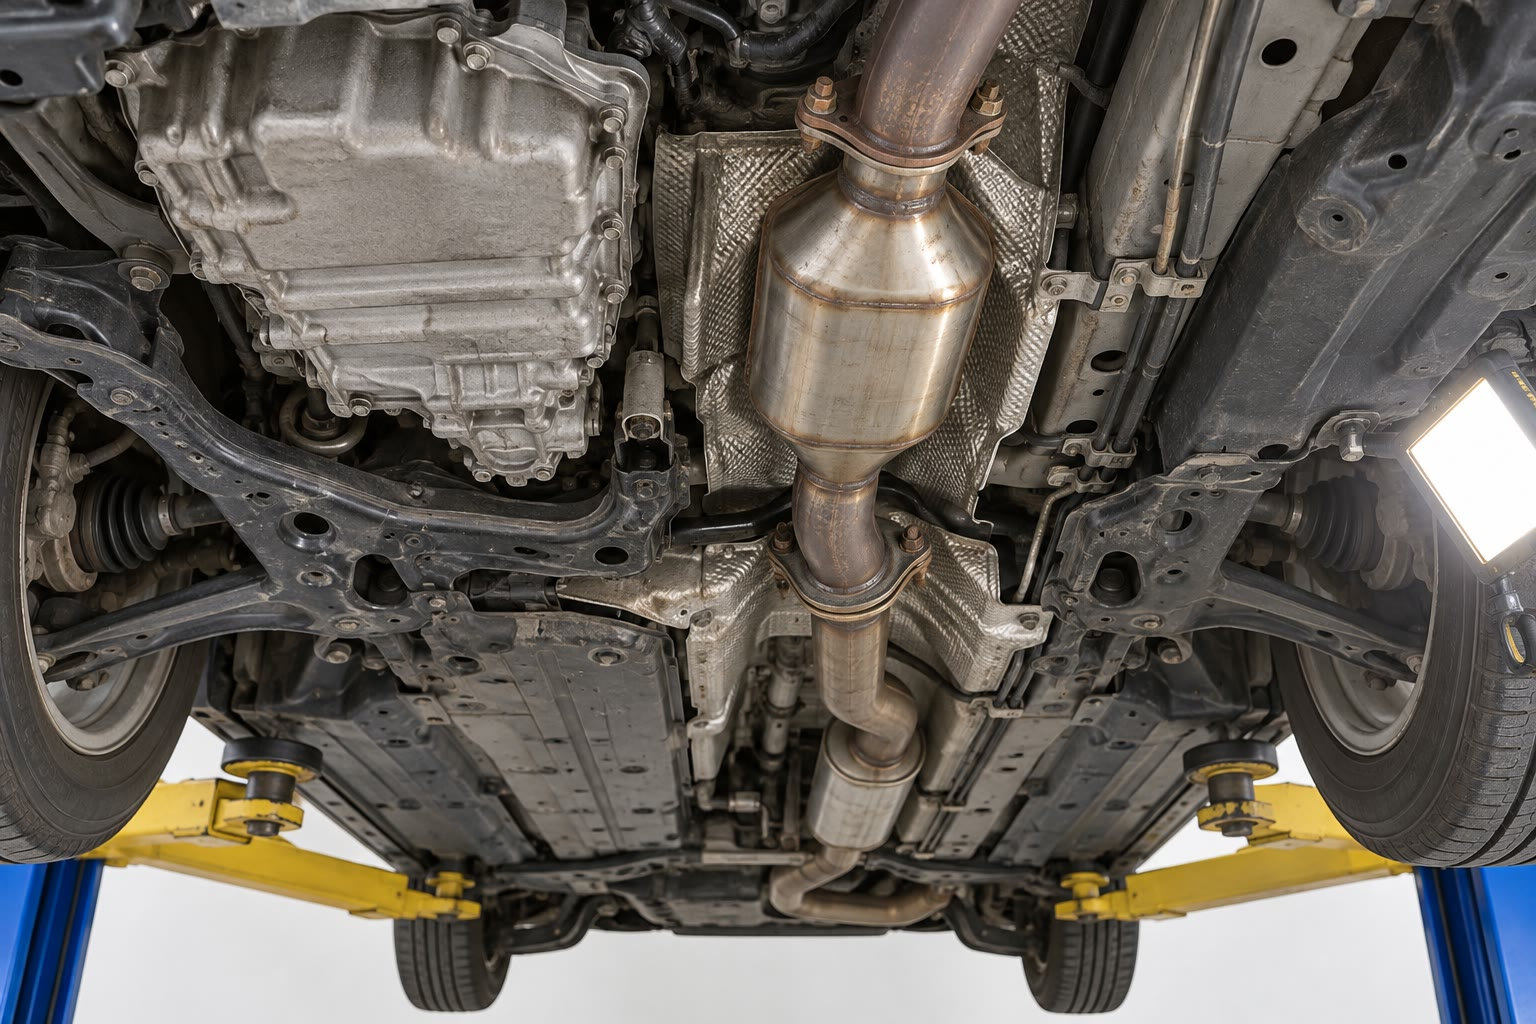
\includegraphics[width=0.5\linewidth]{images/book2/ai/b1-09-catalytic-converter.jpg}

{\small Le dessous d'une voiture~: le boîtier placé sur la ligne
d'échappement est un pot catalytique, un \omterm{def:b1:elementary-steps:catalyst}{catalyseur} hétérogène à la
surface métallique duquel réagissent les gaz d'échappement.}
\end{omfigure}

\begin{definition}[Contrôle cinétique et contrôle thermodynamique]\label{def:b1:elementary-steps:control}
Lorsqu'un réactif peut donner deux produits par des chemins concurrents,
la réaction est sous \emph{contrôle cinétique}\index{controle cinetique@contrôle cinétique} si les proportions des
produits sont fixées par les \omterm{def:b1:rate-laws:rate}{vitesses de formation} (le produit de plus
basse barrière domine), et sous \emph{contrôle
thermodynamique}\index{controle thermodynamique@contrôle thermodynamique} si les chemins sont renversables et que le
système atteint l'équilibre (le produit le plus stable domine).
\end{definition}

\begin{example}[Choisir le produit]\label{ex:b1:elementary-steps:control}
Un réactif donne B en franchissant une barrière de \qty{50}{kJ/mol}
($\Delta E =
\qty{-10}{kJ/mol}$) et C en franchissant une barrière de
\qty{70}{kJ/mol} ($\Delta E =
\qty{-40}{kJ/mol}$). À \qty{300}{K} et aux temps courts, à \omterm{def:b1:rate-laws:activation-energy}{facteurs
préexponentiels} égaux, B se forme $\exp(20000/(8.314 \times 300)) \approx
3000$ fois plus vite que C~: le \omterm{def:b1:elementary-steps:control}{contrôle cinétique} donne B. À haute
température et aux temps longs, B repasse sa petite barrière inverse, C
non, et le système finit sous forme de C~: c'est le \omterm{def:b1:elementary-steps:control}{contrôle
thermodynamique}.
\end{example}

\begin{history}[La catalyse, 1835]
En 1835, le chimiste suédois Jöns Jacob Berzelius réunit sous un même mot
une douzaine d'observations déroutantes --- l'amidon changé en sucre par
les acides, le peroxyde d'hydrogène décomposé par les métaux, l'alcool
oxydé sur le platine --- et appela «~catalytique~» la force cachée à
l'œuvre. Il fallut la cinétique de la fin du siècle, avec Wilhelm
Ostwald, pour définir un \omterm{def:b1:elementary-steps:catalyst}{catalyseur} comme une espèce qui modifie la
vitesse d'une réaction et non son équilibre.
\end{history}

\section{Exercices}

\begin{exercise}[$\star$]\label{exo:b1:elementary-steps:1}
Donner la \omterm{def:b1:elementary-steps:elementary-step}{molécularité} de chaque acte et dire lesquels peuvent être élémentaires~:
(a) $\ce{N2O5 -> NO2 + NO3}$~; (b) $\ce{NO + NO3 -> 2NO2}$~;
(c) $\ce{2H2 + O2 -> 2H2O}$~; (d) $\ce{O + O2 + N2 -> O3 + N2}$.
\end{exercise}

\begin{exercise}[$\star$]\label{exo:b1:elementary-steps:2}
Écrire la \omterm{def:b1:rate-laws:order}{loi de vitesse} des \omterm{def:b1:elementary-steps:elementary-step}{actes élémentaires} $\mathrm{A} + \mathrm{B} \to
\mathrm{C}$, $2\,\mathrm{A} \to \mathrm{B}$ et $\mathrm{A} \to \mathrm{B} +
\mathrm{C}$. Pourquoi ne peut-on pas écrire la \omterm{def:b1:rate-laws:order}{loi de vitesse} d'une
réaction globale à partir de son équation~?
\end{exercise}

\begin{exercise}[$\star$]\label{exo:b1:elementary-steps:3}
Sur le \omterm{def:b1:elementary-steps:energy-profile}{profil énergétique} à deux actes dessiné dans ce chapitre
(intermédiaire à 30, \omterm{def:b1:elementary-steps:energy-profile}{états de transition} à 70 et 55, produits à $-40$,
en \unit{kJ/mol} au-dessus des réactifs), identifier l'intermédiaire,
les \omterm{def:b1:elementary-steps:energy-profile}{états de transition} et l'\omterm{def:b1:elementary-steps:rds}{étape cinétiquement déterminante}. Le
premier acte est-il endothermique ou exothermique~?
\end{exercise}

\begin{exercise}[$\star$]\label{exo:b1:elementary-steps:4}
Un \omterm{def:b1:elementary-steps:catalyst}{catalyseur} multiplie par $10^4$ la \omterm{def:b1:rate-laws:order}{constante de vitesse} directe d'un
\omterm{def:b1:elementary-steps:elementary-step}{acte élémentaire}. Par combien multiplie-t-il la \omterm{def:b1:rate-laws:order}{constante de vitesse}
inverse~? la constante d'équilibre~? la durée nécessaire pour atteindre
l'équilibre~?
\end{exercise}

\begin{exercise}[$\star\star$]\label{exo:b1:elementary-steps:5}
Pour $\mathrm{A} \to \mathrm{B} \to \mathrm{C}$ avec $k_1 =
\qty{0.10}{s^{-1}}$ et $k_2 = \qty{0.30}{s^{-1}}$, calculer $t_{\max}$
et la plus grande concentration de $\mathrm{B}$, en unités de $a_0$.
\end{exercise}

\begin{exercise}[$\star\star$]\label{exo:b1:elementary-steps:6}
Pour $\mathrm{A} \underset{k_{-1}}{\overset{k_1}{\rightleftharpoons}}
\mathrm{I} \xrightarrow{k_2} \mathrm{P}$, tous les actes étant d'ordre 1,
appliquer l'\omterm{def:b1:elementary-steps:qssa}{approximation des états quasi stationnaires} à $\mathrm{I}$
et montrer que $v =
\frac{k_1k_2}{k_{-1} + k_2}[\mathrm{A}]$. Discuter les cas $k_2 \gg
k_{-1}$ et $k_2 \ll k_{-1}$.
\end{exercise}

\begin{exercise}[$\star\star$]\label{exo:b1:elementary-steps:7}
Les ions iodure catalysent la décomposition du peroxyde d'hydrogène~:
\ce{H2O2 + I- -> H2O + IO-} (lent), puis \ce{H2O2 + IO- -> H2O + O2 + I-}
(rapide). Écrire l'équation globale, identifier le \omterm{def:b1:elementary-steps:catalyst}{catalyseur} et
l'intermédiaire, et donner la \omterm{def:b1:rate-laws:order}{loi de vitesse}.
\end{exercise}

\begin{exercise}[$\star\star$]\label{exo:b1:elementary-steps:8}
Un acte forme un carbocation à partir d'une molécule neutre, processus
fortement endothermique. À l'aide du postulat de Hammond, expliquer
pourquoi un substituant qui stabilise le carbocation accélère aussi
l'acte.
\end{exercise}

\begin{exercise}[$\star\star$]\label{exo:b1:elementary-steps:9}
Dans l'\cref{ex:b1:elementary-steps:control}, calculer le rapport des
constantes de \omterm{def:b1:rate-laws:rate}{vitesse de formation} de B et de C à \qty{300}{K} et à
\qty{600}{K}. Commenter.
\end{exercise}

\begin{exercise}[$\star\star\star$]\label{exo:b1:elementary-steps:10}
Un gaz $\mathrm{A}$ se décompose après avoir été activé par un choc avec
une molécule quelconque $\mathrm{M}$~: $\mathrm{A} + \mathrm{M} \rightleftharpoons
\mathrm{A}^* + \mathrm{M}$ ($k_1$, $k_{-1}$), puis $\mathrm{A}^* \to
\mathrm{P}$ ($k_2$). À l'aide de l'\omterm{def:b1:elementary-steps:qssa}{approximation des états quasi
stationnaires} appliquée à
$\mathrm{A}^*$, déterminer $v$, et montrer que la réaction est d'ordre 1
à haute pression et d'ordre 2 à basse pression.
\end{exercise}

\begin{exercise}[$\star\star\star$]\label{exo:b1:elementary-steps:11}
Démontrer la formule de $[\mathrm{B}](t)$ du
\cref{thm:b1:elementary-steps:consecutive} et traiter le cas particulier
$k_1 = k_2 = k$, pour lequel $[\mathrm{B}] = a_0kt\,\eu^{-kt}$.
\end{exercise}

\begin{exercise}[$\star\star\star$]\label{exo:b1:elementary-steps:12}
La réaction globale $\mathrm{A} + 2\,\mathrm{B} \to \mathrm{P} +
\mathrm{C}$ a pour \omterm{def:b1:rate-laws:order}{loi de vitesse} expérimentale $v =
k[\mathrm{A}][\mathrm{B}]^2/[\mathrm{C}]$. Proposer un mécanisme
comportant un pré-équilibre rapide qui l'explique.
\end{exercise}

\section{Problème~: pourquoi le monoxyde d'azote s'oxyde plus vite à froid}

\begin{problem}[{Problème du week-end --- l'oxydation d'ordre trois du
monoxyde d'azote, un pré-équilibre passant par le dimère \ce{N2O2}, le
traitement par l'état quasi stationnaire, et une \omterm{def:b1:rate-laws:activation-energy}{énergie d'activation}
apparente négative}]
\label{pb:b1:elementary-steps:1}
Pour \ce{2NO(g) + O2(g) -> 2NO2(g)}, des mesures de \omterm{def:b1:rate-laws:initial-rate}{vitesse initiale} à
\qty{300}{K} donnent (vitesses en \unit{mol.L^{-1}.s^{-1}})~:
\begin{center}
\begin{tabular}{cccc}
\hline
expérience & $[\ce{NO}]_0$ (mol/L) & $[\ce{O2}]_0$ (mol/L) & $v_0$ \\
\hline
1 & \num{1.0e-3} & \num{1.0e-3} & \num{1.0e-5} \\
2 & \num{2.0e-3} & \num{1.0e-3} & \num{4.0e-5} \\
3 & \num{1.0e-3} & \num{2.0e-3} & \num{2.0e-5} \\
\hline
\end{tabular}
\end{center}
La \omterm{def:b1:rate-laws:order}{constante de vitesse} trouvée à \qty{400}{K} est dix fois plus petite
qu'à \qty{300}{K}. Prendre $R = \qty{8.314}{J/(mol.K)}$.
Le mécanisme proposé est
\[
  \ce{2NO <=> N2O2} \ \ (k_1, k_{-1}, \text{rapide}), \qquad
  \ce{N2O2 + O2 -> 2NO2} \ \ (k_2, \text{lent}).
\]

\medskip
\noindent\textbf{Partie I --- La loi observée.}
\begin{enumerate}
  \item Déterminer les \omterm{def:b1:rate-laws:order}{ordres partiels} par rapport à \ce{NO} et à \ce{O2}.
  \item Écrire la \omterm{def:b1:rate-laws:order}{loi de vitesse} et calculer $k$ à \qty{300}{K}, avec son
        unité.
  \item La réaction pourrait-elle être un acte trimoléculaire unique~?
        Donner un argument.
  \item Calculer l'\omterm{def:b1:rate-laws:activation-energy}{énergie d'activation} apparente à partir des deux
        températures.
  \item Pourquoi une \omterm{def:b1:rate-laws:activation-energy}{énergie d'activation} négative est-elle impossible
        pour un \omterm{def:b1:elementary-steps:elementary-step}{acte élémentaire}~?
  \item Écrire les \omterm{def:b1:rate-laws:rate}{vitesses de disparition} de \ce{NO} et de \ce{O2} en
        fonction de $v$.
\end{enumerate}

\medskip
\noindent\textbf{Partie II --- Le pré-équilibre.}
\begin{enumerate}[resume]
  \item Vérifier que les deux actes ont pour somme la réaction globale.
        Nommer l'intermédiaire.
  \item Donner la \omterm{def:b1:elementary-steps:elementary-step}{molécularité} de chaque acte.
  \item Écrire la vitesse de l'acte lent.
  \item Exprimer $[\ce{N2O2}]$ à l'aide de l'\omterm{def:b1:elementary-steps:pre-equilibrium}{approximation du
        pré-équilibre rapide}.
  \item En déduire la \omterm{def:b1:rate-laws:order}{loi de vitesse} et comparer à l'expérience.
  \item Exprimer la constante observée à l'aide de $k_1$, $k_{-1}$ et
        $k_2$.
\end{enumerate}

\medskip
\noindent\textbf{Partie III --- L'état quasi stationnaire.}
\begin{enumerate}[resume]
  \item Écrire $\dd[\ce{N2O2}]/\dd t$ pour le mécanisme complet.
  \item Appliquer l'\omterm{def:b1:elementary-steps:qssa}{approximation des états quasi stationnaires} et
        exprimer $[\ce{N2O2}]$.
  \item En déduire la \omterm{def:b1:rate-laws:order}{loi de vitesse} $v = \dfrac{k_1k_2[\ce{NO}]^2[\ce{O2}]}{k_{-1} +
        k_2[\ce{O2}]}$.
  \item Dans quelle limite se réduit-elle au résultat de la partie II~?
  \item Que deviendraient les ordres dans la limite opposée~?
  \item Quelle limite les mesures de la partie I confirment-elles~?
\end{enumerate}

\medskip
\noindent\textbf{Partie IV --- L'\omterm{def:b1:rate-laws:activation-energy}{énergie d'activation} apparente.}
Chaque acte suit la \omterm{thm:b1:rate-laws:arrhenius}{loi d'Arrhenius}, avec les \omterm{def:b1:rate-laws:activation-energy}{énergies d'activation}
$E_1 =
\qty{2}{kJ/mol}$, $E_{-1} = \qty{40}{kJ/mol}$ et $E_2 =
\qty{15}{kJ/mol}$.
\begin{enumerate}[resume]
  \item Écrire $\ln k$ en fonction des logarithmes de $k_1$, $k_{-1}$ et
        $k_2$.
  \item En déduire $E_a = E_1 - E_{-1} + E_2$.
  \item Interpréter~: pourquoi une combinaison d'\omterm{def:b1:elementary-steps:elementary-step}{actes élémentaires}
        peut-elle avoir une \omterm{def:b1:rate-laws:activation-energy}{énergie d'activation} apparente négative~?
  \item Esquisser le \omterm{def:b1:elementary-steps:energy-profile}{profil énergétique}~: où se trouve le second \omterm{def:b1:elementary-steps:energy-profile}{état de
        transition} par rapport aux réactifs \ce{2NO + O2}~?
  \item De quel facteur la vitesse varierait-elle entre 300 et
        \qty{400}{K} avec cette valeur~?
  \item Calculer l'\omterm{def:b1:rate-laws:activation-energy}{énergie d'activation} apparente à partir des valeurs
        relatives aux actes, et comparer à la partie I.
\end{enumerate}
\end{problem}
